\documentclass{article}

\usepackage{arxiv}

\usepackage[utf8]{inputenc} % allow utf-8 input
\usepackage[T1]{fontenc}    % use 8-bit T1 fonts
\usepackage{lmodern}        % https://github.com/rstudio/rticles/issues/343
\usepackage{hyperref}       % hyperlinks
\usepackage{url}            % simple URL typesetting
\usepackage{booktabs}       % professional-quality tables
\usepackage{amsfonts}       % blackboard math symbols
\usepackage{nicefrac}       % compact symbols for 1/2, etc.
\usepackage{microtype}      % microtypography
\usepackage{graphicx}

\title{How much gut content data is required to predict trophic
interactions?}

\author{
    Anubhav Gupta
    \thanks{Corresponding author}
   \\
    Department of Evolutionary Biology and Environmental Studies \\
    University of Zurich \\
  8057 Zurich, Switzerland \\
  \texttt{\href{mailto:anubhav.gupta@ieu.uzh.ch}{\nolinkurl{anubhav.gupta@ieu.uzh.ch}}} \\
   \And
    Eoin O' Gorman
   \\
    School of Life Sciences \\
    University of Essex \\
  CO4 3SQ Colchester, UK \\
  \texttt{\href{mailto:e.ogorman@essex.ac.uk}{\nolinkurl{e.ogorman@essex.ac.uk}}} \\
   \And
    Other authors
   \\
    XXX XXX \\
    XXX XXX \\
  XXX XXX \\
  \texttt{XXX XXX} \\
   \And
    Owen L. Petchey
   \\
    Department of Evolutionary Biology and Environmental Studies \\
    University of Zurich \\
  8057 Zurich, Switzerland \\
  \texttt{\href{mailto:owen.petchey@ieu.uzh.ch}{\nolinkurl{owen.petchey@ieu.uzh.ch}}} \\
  }


% tightlist command for lists without linebreak
\providecommand{\tightlist}{%
  \setlength{\itemsep}{0pt}\setlength{\parskip}{0pt}}


% Pandoc citation processing
\newlength{\cslhangindent}
\setlength{\cslhangindent}{1.5em}
\newlength{\csllabelwidth}
\setlength{\csllabelwidth}{3em}
\newlength{\cslentryspacingunit} % times entry-spacing
\setlength{\cslentryspacingunit}{\parskip}
% for Pandoc 2.8 to 2.10.1
\newenvironment{cslreferences}%
  {}%
  {\par}
% For Pandoc 2.11+
\newenvironment{CSLReferences}[2] % #1 hanging-ident, #2 entry spacing
 {% don't indent paragraphs
  \setlength{\parindent}{0pt}
  % turn on hanging indent if param 1 is 1
  \ifodd #1
  \let\oldpar\par
  \def\par{\hangindent=\cslhangindent\oldpar}
  \fi
  % set entry spacing
  \setlength{\parskip}{#2\cslentryspacingunit}
 }%
 {}
\usepackage{calc}
\newcommand{\CSLBlock}[1]{#1\hfill\break}
\newcommand{\CSLLeftMargin}[1]{\parbox[t]{\csllabelwidth}{#1}}
\newcommand{\CSLRightInline}[1]{\parbox[t]{\linewidth - \csllabelwidth}{#1}\break}
\newcommand{\CSLIndent}[1]{\hspace{\cslhangindent}#1}

\usepackage{lineno}
\usepackage {amsmath}
\setlength\parindent{24pt}
\usepackage{setspace}\doublespacing
\begin{document}
\maketitle


\begin{abstract}
\begin{enumerate}
\def\labelenumi{\arabic{enumi})}
\tightlist
\item
  One of the biggest obstacles in food web ecology is the time and
  effort required to adequately describe the structure of a food web
  using gut content data. Food web models such as the ADBM can be used
  to circumvent this problem by predicting the interactions based on
  easily measured characteristics, such as the size of organisms.
  However, presence-absence data such as gut content data is required to
  parameterise these food web models. And collecting and analysing these
  data from the field is an expensive and time consuming task.
  Therefore, it is crucial to know how much gut content data is required
  to parameterise food web models with high accuracy and high precision.
\item
  Here, we explore seven food webs in the literature and determine how
  much gut content data would be needed to accurately predict their
  structure using the ADBM. We use Bayesian computation to parameterise
  the ADBM, and true skill statistics to measure the goodness of fit,
  and do so while varying the amount of gut content data used in the
  parameterisation.
\item
  We estimated the minimum amount of gut content data required for seven
  different food webs that resulted in 95\% of the maximum true skill
  statistics achieved by the ADBM when all available gut content data
  was used. We found that incomplete gut content data can be used to
  parameterise the ADBM with the lowest amount of gut content data being
  28\% of the available gut content data.
\item
  These results suggest that one need not collect such a large quantity
  of gut content data to predict the structure of a food web, thereby
  reducing sampling effort considerably, while having little effect on
  precision or accuracy of predictions.
\end{enumerate}
\end{abstract}

\keywords{
    gut content data
   \and
    ADBM
   \and
    food web accuracy
   \and
    food web prediction
  }

\hypertarget{introduction}{%
\section{Introduction}\label{introduction}}

Knowledge about the trophic interactions in a food web is crucial in
ecology for purposes ranging from identifying keystone species (Jord'an
2009) to quantifying robustness of a food web to species extinctions
(Dunne, Williams, and Martinez 2002). This has led to the development of
numerous food web models (Allesina, Alonso, and Pascual 2008; Cohen,
Newman, and Steele 1985; Gravel et al. 2013; Petchey et al. 2008;
Tamaddoni-Nezhad et al. 2013). Along with inferring missing links in an
observed food web, the food web models are also used for ecological
forecasting (Hattab et al. 2016; Lindegren et al. 2010) and for
understanding the underlying mechanism governing the interactions in a
food web (Gorman et al. 2019).

Although food web models are constructed using prior theory about the
factors that determine trophic interactions, empirical data about
interactions is required to parameterise a model. For example, Petchey
et al. (2008) used presence-absence information about trophic
interactions to parameterise the allometric diet breadth model and
thereby predict species interactions. These empirical information about
interactions can come from diverse set of methods such as gut content
analysis (Peralta-Maraver, Lopez-Rodriguez, and de Figueroa 2017),
stable isotope ratio analysis of tissues (Layman et al. 2007),
experimentation (Warren 1989), DNA metabarcoding of gut contents or
faeces (Roslin and Majaneva 2016) and literature research (Gray et al.
2015; Cohen and Mulder 2014a; Goldwasser and Roughgarden 1993a).

Each of these sources of information about trophic interactions has
shortcomings. For example: Stable isotope ratio analysis of the
organism's tissue does not give direct information of the diet of that
organism but rather gives approximate trophic position of that species
in the food web (Wada, Mizutani, and Minagawa 1991; Jennings and van der
Molen 2015). Although mixing models can be used to determine what prey
items are most likely fed upon by a predator, this results in
uncertainty in the estimates (Kadoya, Osada, and Takimoto 2012;
Crawford, Mcdonald, and Bearhop 2008). Similarly, DNA metabarcoding
could have issues in detecting secondary predation or cannibalism
(Pompanon et al. 2012; Nielsen et al. 2018) and is prone to
environmental contamination (e.g.~DNA in the water swallowed along with
DNA from an aquatic consumer's prey cannot be differentiated from actual
prey) (Kelly et al. 2014). Furthermore, construction of food webs via
literature review can lead to false positives--links included when in
reality no link would occur because it makes an assumption that the
species interactions inferred from a system will occur in another system
as well(Gray et al. 2015; Cohen and Mulder 2014b; Goldwasser and
Roughgarden 1993b).

Nielsen et al. (2018) have shown that gut content analysis method has a
better match with real diet when compared to other methods.

Acquiring food web data from gut content analysis is time consuming and
expensive (AG: Do we need a reference? Next sentence explains the
reason.). In part this is due to the perception that many gut contents
must be collected and analysed in order to be confident that the
majority of possible trophic links among species have been observed.
Furthermore, considerable time, resource investment, and expertise is
required to process the collected samples. Hence, there is of
considerable importance to know the minimum number of gut contents and
of which consumer species that are required to parameterise a food web
model with high accuracy and high precision, so that one knows when is a
good time to stop collecting any further empirical data on the food web.

Therefore, the key question we are interested in answering is how much
presence-absence information, in the form of gut content data, is
required to infer food web structure from a food web model with high
accuracy and high precision. In other words, how many samples of gut
content should one collect from the field to parameterise a food web
model? To answer this question, we use the presence-absence information
from gut content data to parameterise the allometric diet breadth model
(ADBM) thereby predicting trophic interactions in seven different food
webs using rejection approximate Bayesian computation, where the fit of
the model was measured using true skill statistics. We computed the true
skill statistics of the predicted food webs for different number of
predator guts to calculate the minimum number of gut content data to
infer food web structure. Our study provides a guideline on how many gut
content data is required to predict food web structure using a food web
model.

\hypertarget{materials-and-methods}{%
\section{Materials and Methods}\label{materials-and-methods}}

In the upcoming sections, we present the empirical food webs, the
allometric diet breadth model (ADBM), and the gut content data used to
infer the trophic interactions. We also give a detailed account of using
partial gut content data to parameterise the ADBM using rejection
approximate Bayesian computation (ABC). We assessed model predictions
using the true skill statistic for comparison across food webs.

\hypertarget{the-empirical-food-webs}{%
\subsection{The Empirical Food Webs}\label{the-empirical-food-webs}}

In our study, we used food webs for which gut content data is available
at an individual level and data that is or that we could make FAIR
(Wilkinson et al. 2016). Presence and absence interactions of food web
data can be aggregated in different ways (Gilljam et al. 2011). A common
way of aggregating food web data is the taxonomic approach, in which
nodes in the food web are taxa (e.g.~species), or life stages of taxa,
and one species is said to feed on another species if at least one
individual of the latter is found in at least one gut of the former.
Another approach is based on size, rather than taxonomy, and in this the
nodes in the food web are size classes. Here, a feeding link occurs
between two size classes if at least one prey item within a size class
was found in the gut of another size class, irrespective of their
taxonomy.

In our study, we aggregate the gut content data on the basis of size
class because the food webs constructed using this approach were better
predicted by the ADBM compared to the taxonomic approach (Woodward et
al. 2010a), and this is because the ADBM is based on foraging rules
defined using the body sizes of organisms (Petchey et al. 2008).

Our study is based on the assumption that the food web constructed using
the complete gut content data is the true food web. However, this might
not be the case because the links are still under-sampled for many nodes
(Woodward et al. 2010b). This could result in a lower true skill
statistic (TSS) of the predicted food web from the ADBM, which can
result in a biased estimate of the minimum number of gut content data
required to achieve 95\% of the TSS achieved using complete gut content
data.

In the following sections 2.1.1-2.1.5, we briefly explain seven
empirical food webs used in our study. The text used in those sections
are paraphrased from Gilljam et al. (2011).

\hypertarget{broadstone-stream}{%
\subsubsection{Broadstone Stream}\label{broadstone-stream}}

Broadstone Stream (51\(^\circ\) 05' N 0\(^\circ\) 03' E; 120 m above
sea-level) is a second-order tributary of the River Medway in south-east
England. At the time of sampling in 1996--1997, the stream was acidic
(pH 4.7--6.6) and fishless. About 31 common species make up the
macroinvertebrate food web, including six major predators and
detritivores like stoneflies and chironomids (Woodward, Speirs, and
Hildrew 2005).

Between June 1996 and April 1997, thirty randomly scattered benthic
Surber sample-units (25cm \(\times\) 25cm quadrat; mesh aperture 330mm)
were taken every two months and kept in 5\% formalin. All individuals
retrieved from the benthos and identified in stomach contents had their
linear body dimensions quantified and converted to dry mass using known
regression formulae (listed in Woodward and Hildrew (2002)).

The predators' foreguts were dissected and analysed with 400
magnification in the Surber samples. The individual body masses of eaten
prey were calculated using the same methods as for the benthic samples,
using reference slides as a guide (Woodward, Speirs, and Hildrew 2005).
Over the six sample instances, a single dataset was produced. Each
predator and prey individual involved in a feeding relationship was
measured and converted into their respective body masses, resulting in a
total of 2893 individuals.

\hypertarget{celtic-sea}{%
\subsubsection{Celtic Sea}\label{celtic-sea}}

The Celtic Sea is a continental shelf area that is bounded by Ireland,
the United Kingdom, and the Bay of Biscay. Because the Barnes et al.
(2008) dataset, from which the data utilised in this chapter were taken,
did not provide precise sampling sites and dates, the data was pooled
throughout the whole time period and locations to capture broad
tendencies. Only places that were sampled consistently from 1987 to 2001
were used (Blanchard et al. 2005).

In a published global dataset of individual predator and prey body sizes
and taxonomy (Barnes et al., 2008), the feeding linkages of fish in the
Celtic Sea were described. The original stomach contents data were
acquired during annual surveys conducted by the Centre for Environment,
Fisheries, and Aquaculture Science (Cefas) on board research vessels
during dissections (Pinnegar et al. 2003). Barnes et al. (2008) used
known regression equations to measure predator and prey lengths and
convert them to body mass.

\hypertarget{afon-hirnant}{%
\subsubsection{Afon Hirnant}\label{afon-hirnant}}

Three sites in the Afon Hirnant, in North Wales, UK (\(52^\circ\) 52' N
\(03^\circ\) 34' W), were used for the study. The average yearly
discharge was 2.08 to 7.26 \(m^3/s\), with a pH ranging from 5.5 to 7.
(check Figueroa (2007) and Woodward et al. (2010c) for full details).
Invertebrates were collected using a Hess sampler (sampling area: 0.028
\(m^2\); mesh aperture 80 \(\mu m\)), with 15 sample-units obtained at
random at each site and season, totaling 180 samples across the sampling
period. The invertebrate fauna was promptly preserved in 100\% ethanol
and sorted in the lab. By removing predators' foreguts, which were
mounted in Euparal media and viewed at 400 magnification, feeding
interactions were determined.

Every predator's linear dimensions (for example, body length) and
individual prey items inside each predator's foregut were measured and
then translated to body mass values using published regression equations
for each taxon (presented in Woodward et al. (2010c)). If the prey items
were highly digested, the average body length of individuals in the same
family (Ephemeroptera, Plecoptera, or Trichoptera) in the habitat was
used. The body lengths of Chironomidae (Diptera) were calculated using
previously established species-specific regressions between head capsule
width and body length (Figueroa 2007).

\hypertarget{tadnoll-brook}{%
\subsubsection{Tadnoll Brook}\label{tadnoll-brook}}

The Tadnoll Brook is a tributary of the River Frome in Southern England,
UK, with a mean annual discharge of 0.35 \(m^3/s\) and a pH of 6.9--7.7.
(Edwards et al., 2009b).

A 240-m reach was sampled every two months between February and December
2005 to create the summary food web. A Surber sampler was used to
collect invertebrates every two months (0.06 m2; mesh aperture 300 mm).
20 random samples were taken on each occasion, stored in the field in
4\% (w/v) formalin, and then sorted for invertebrates. Fish were
captured with an electrofisher, anaesthetized with 2-phenoxyethanol,
recognised to species, measured, and weighed on each occasion (Woodward
et al., 2010). The guts of trout (Salmo trutta L.) with fork lengths
more than 70 mm were then flushed with a tiny manual water pump and
stored in 4\% formalin. For smaller trout and other fish species
(\emph{Cottus gobio}, \emph{Anguilla anguilla}, \emph{Phoxinus
phoxinus}, \emph{Barbatula barbatula}, \emph{Gasterosteus aculeatus}),
specimens were sacrificed and frozen for subsequent dissection.

Gut contents analysis was performed on each sample occasion for the fish
assemblage, whereas invertebrates had far less varied diets and were
only characterised in May and October. Individuals of the benthos'
numerically dominant or trophically important invertebrate taxa were
taken from the Surber samples, dissected, and the contents of the
foregut investigated for animal prey, which were recognised at
\(400\times\) magnification by comparison with reference specimens. The
taxa used to examine stomach contents covered more than 95\% of the
individuals observed in the Benthos. Wherever possible, predators' gut
contents were matched to species, and linear body dimensions were
measured. Using established regression equations, the dry mass of prey
items and invertebrate predators was calculated (Benke et al. 1999;
Ganihar 1997; Burgherr and Meyer 1997; Gonzalez, Basaguren, and Pozo
2002; Smock 1980; Edwards et al. 2009; MEYER 1989).

\hypertarget{guampoe-coilaco-and-trancura-rivers-chile}{%
\subsubsection{Guampoe, Coilaco and Trancura Rivers,
Chile}\label{guampoe-coilaco-and-trancura-rivers-chile}}

Three rivers (the Coilaco, Guampoe, and Trancura Rivers) in the
catchment area of the Tolten River in south Chile, South America, were
studied in a similar way. The Coilaco River (discharge 2.1--16.8
\(m^3/s\)), Guampoe River (output 1.8--7.5 \(m^3/s\)), and Trancura
River (discharge 8.8--49.3 \(m^3/s\)) are all pH 6.7--7.6 circumneutral
rivers (Figueroa 2007).

In each river, eight benthic samples were taken in each season between
1984 and 1985, totaling 96 sample-units for the whole sampling period
(Campos et al., 1985). Invertebrates were gathered using a Surber
sampler (sampling area: 0.09 \(m^2\); mesh aperture 250 \(\mu m\)) and
stored in 70\% ethanol before being transported to the lab for species
identification and food web analysis.

The feeding linkages were discovered by analysing the gut contents of
all individuals observed in each sample. Large invertebrates had their
guts removed and mounted in Euparal, whilst small specimens were mounted
whole and studied with \(400\times\) magnification. Following Schmid
(1993) and (Schmid-Araya et al. 2002), species prey items detected on
each gut were identified using previously mounted reference slides.
Using known regression equations (mentioned in Reiss and Schmid-Araya
(2008); Baumgärtner and Rothhaupt (2003); Miserendino (2001); Woodward
et al. (2010b)), all linear dimensions were translated to body mass
estimates.

\hypertarget{allometric-diet-breadth-model-adbm}{%
\subsection{Allometric Diet Breadth Model
(ADBM)}\label{allometric-diet-breadth-model-adbm}}

The allometric diet breadth model (ADBM) is based on optimal foraging
theory, specifically the contingency foraging model (MacArthur and
Pianka 1966). We chose this model for various reasons, including because
it uses the body size of organisms as input to predict feeding
interactions, and because of our familiarity with it. The ADBM predicts
the set of prey types (e.g.~species or sizes classes) a consumer should
feed upon to maximise its rate of energy intake (Petchey et al. 2008).
The foraging variables in the model are: energy content of the
resources, handling times of the prey, space clearance rate, and prey
densities. These are allometrically scaled to the body sizes of the
species. Further details on the foraging rules defined in the ADBM and
ADBM's predictive power across different food webs can be found in
Petchey et al. (2008).

\hypertarget{assessment-of-prediction}{%
\subsection{Assessment of prediction}\label{assessment-of-prediction}}

The accuracy of the predicted diet of the predators was measured using
true skill statistic (TSS) which takes into account the true and false
predictions of both the presence and absence of links defined as:

\[ \text{TSS} = \frac{ad-bc}{(a+c)(b+d)} \] where \(a\) is the number of
observed links that are predicted by the model (true positives), \(d\)
is the number of observed absences of links that are correctly predicted
(true negatives), \(b\) is the number of false positives, and \(c\) is
the number of false negatives. The \(TSS\) ranges from \(-1\) to \(1\),
where +1 indicates a perfect prediction. A \(TSS\) value of zero or less
indicates a performance no better than random (Allouche, Tsoar, and
Kadmon 2006).

\hypertarget{inferring-food-web-using-partial-gut-content-data}{%
\subsection{Inferring food web using partial gut content
data}\label{inferring-food-web-using-partial-gut-content-data}}

\textbf{Comment AG: Is it necessary to have the sections 1.1 and 1.2 of
the supplementary information in the Supplementary information or shall
the sections 1.1 and 1.2 be migrated to the main text (manuscript)?}

From an empirical dataset of gut content data, we take a random sample
of gut contents of specific size (see below) to create a partial gut
content dataset. We then fit the ADBM to this partial dataset.

\begin{figure}

{\centering 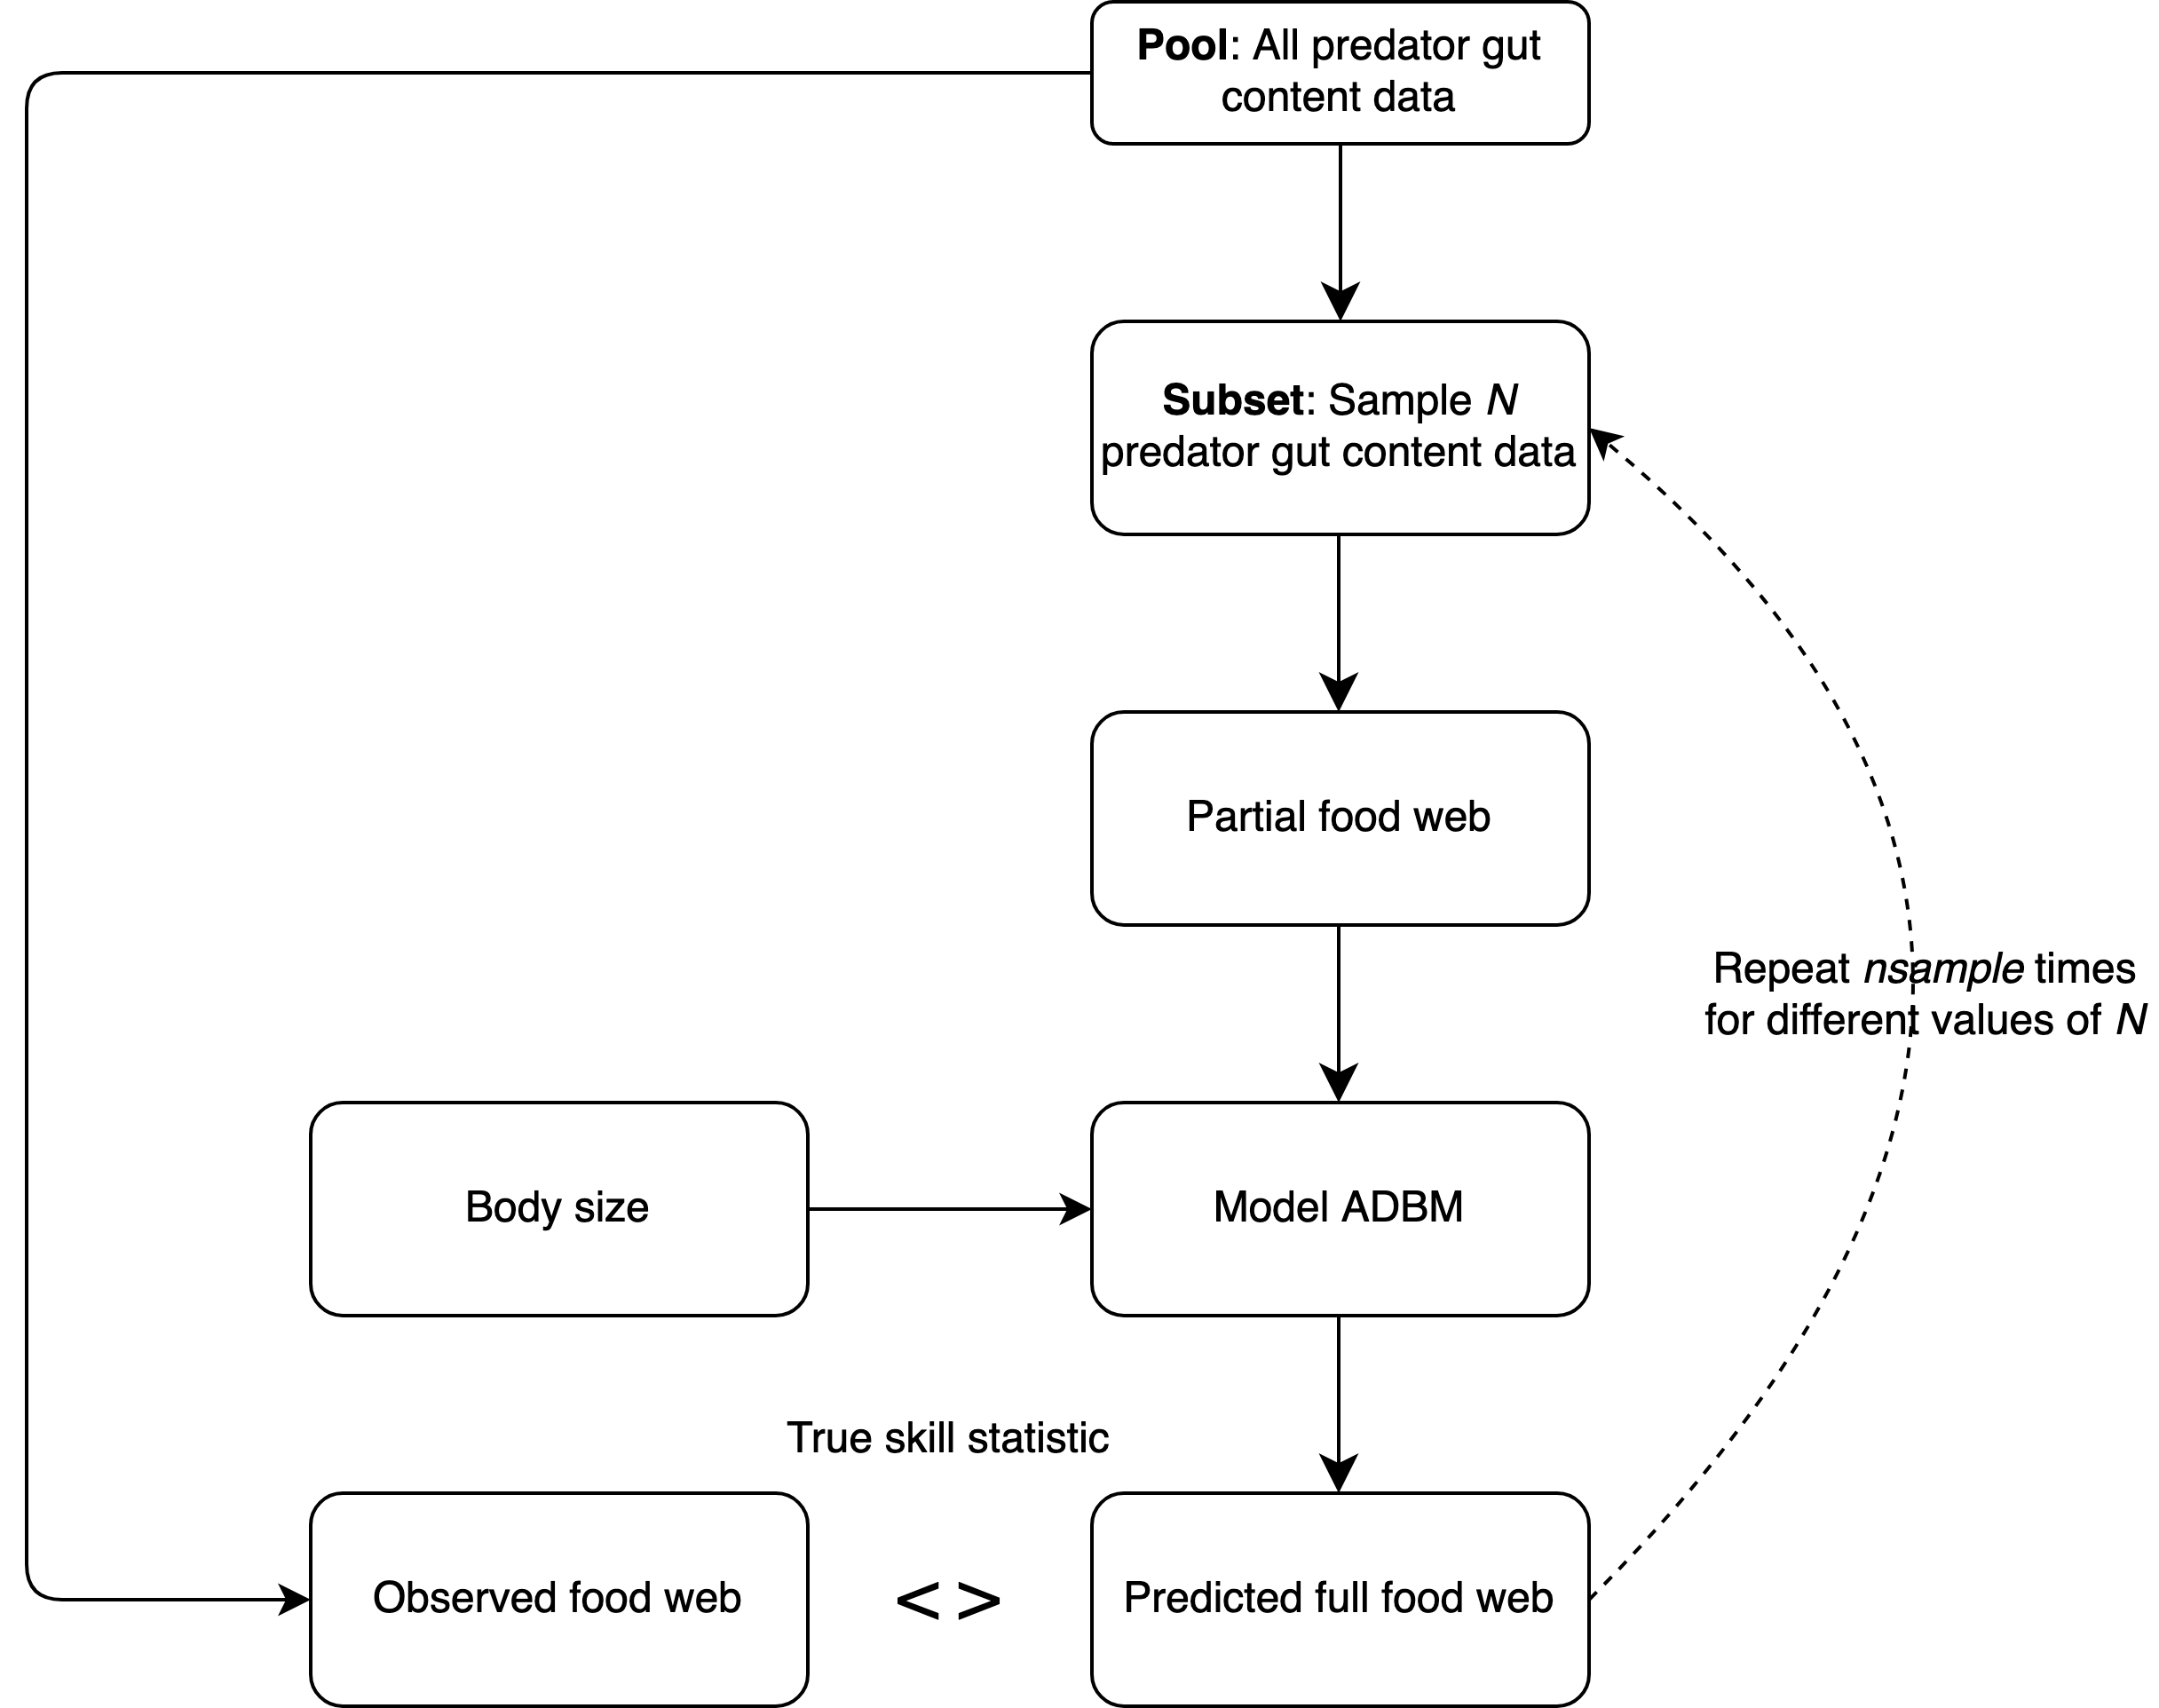
\includegraphics[width=500px]{../../manuscript/fig/ms_C2(1)} 

}

\caption{\label{fig:fig_ra} (a, c, e, g, i, k, m) Accuracy of the predicted food web measured using the true skill statistics, predicted by the ADBM parameterised using gut content data. Line and shaded grey region represents the mean and the prediction interval of 100 independent samples respectively. Red line represents the number of predator guts required to achieve a TSS of 95\% of the maximum TSS. (b, d, f, h, j, l, n) Ratio of the true skill statistic of the predicted food web by the ADBM parameterised using gut content data to that of the predicted food web constructed using gut content data only. The dashed line shows where the ratio is one for reference.}\label{fig:unnamed-chunk-1}
\end{figure}

To fit the ADBM to a gut content dataset (be it complete or partial), we
used the rejection ABC method we previously developed in Gupta, Furrer,
and Petchey (2022) to accept a parameter value from a prior distribution
which would have resulted in the minimum distance, where distance = 1 -
True skill statistic. The true skill statistic was computed between the
diets predicted from the ADBM, and those observed in the sampled gut
content data. We repeated this process \(n~(= 100)\) times for every
\(i\) number of guts, where \(i\) lies between 1 and total number of gut
content data in the pool.

\emph{Input:}

\begin{itemize}
\item
  Predators \(P: P = \{p_1, p_2, \dots, p_k \}\)
\item
  A pool of gut content data \(G: G = \{g_1, g_2, \dots, g_n\}\), where
  \(g_{n}\) is the observed diet matrix containing ones and zeros.
\item
  A model prediction
  \(model(\theta): ADBM(\theta) = \{d_{p_1}, d_{p_1}, \dots, d_{p_k}\}\),
  where \(d_{p_k}\) is the predicted diet matrix of predator \(k\)
  containing ones and zeros.
\item
  A summary statistic \(s(x): s(x) \subseteq model(\theta)\), where
  \(s(x)\) is the diet of some or all of the predators.
\item
  A distance function \(d(x_i, y) : d(x_i,y) = 1 - TSS(x_i, y)\), which
  quantifies how close the observed diet is to the predicted diet of
  some or all of the predators.
\item
  An observed food web
  \(Y: Y = \{d_{p_1}', d_{p_1}', \dots, d_{p_k}'\}\), where \(d_{p_k}'\)
  is the observed diet matrix of predator \(k\) containing ones and
  zeros.
\end{itemize}

\emph{Sampling:}

for \(i = 1, \dots, tgut\) where \(tgut\) is the total number of gut
content data in the pool \(G\)

\begin{itemize}
\item
  for \(j = 1, \dots, nsample\) where \(nsample\) is the number of
  independent samples to be drawn

  \begin{itemize}
  \item
    Draw a set of gut content data \(y = \{g_1, g_2, \dots, g_i\}\) from
    the pool of gut content data \(G\)
  \item
    for \(k = 1, \dots, npar\) where \(npar\) is the number of parameter
    values to be sampled

    \begin{itemize}
    \item
      Draw a set of parameter values \(\theta_k\) from the prior
      distribution \(\pi(\theta)\)
    \item
      Compute the model result \(x_i = model(\theta_k)\)
    \item
      Compute \(s(x_i)\) and \(d(s(x_i), y)\)
    \end{itemize}
  \item
    Accept \(\theta_j\), which results in the \(min_i\{d(s(x_i), y)\}\)
  \end{itemize}
\item
  Compute
  \(TSS_{i}(x, y) = \{TSS(x_i,y): x_i = ADBM(\theta_j), \theta_j \text{ computed from previous step}\}\)
  using the accepted \(\theta_1, \dots, \theta_{nsample}\)
\end{itemize}

\emph{Output:}

The \(TSS\) between observed and predicted food webs, and the posterior
parameter distributions for every \(i\) number of gut content data drawn
from the pool of gut content data.

\hypertarget{computing-the-minimum-gut-content-data}{%
\subsection{Computing the minimum gut content
data}\label{computing-the-minimum-gut-content-data}}

Using TSS of the predicted food webs for different number of predator
guts, we computed the number of gut content data that results in the
mean TSS equal to the 95\% of the mean TSS achieved by the model using
all the predator guts for a food web. We call this number of gut content
data as the minimum gut content data.

\hypertarget{results}{%
\section{Results}\label{results}}

We first present how the accuracy of the food web model in predicting
trophic interactions varies with increasing amount of gut content data
provided to the food web model. Then, we calculate the number of gut
content data for each food webs that results in accuracy equal to 95\%
of the maximum true skill statistics predicted by the food web model.

\hypertarget{inferring-trophic-interactions-using-adbm-and-incomplete-gut-content-data}{%
\subsection{Inferring trophic interactions using ADBM and incomplete gut
content
data}\label{inferring-trophic-interactions-using-adbm-and-incomplete-gut-content-data}}

\begin{figure}

{\centering 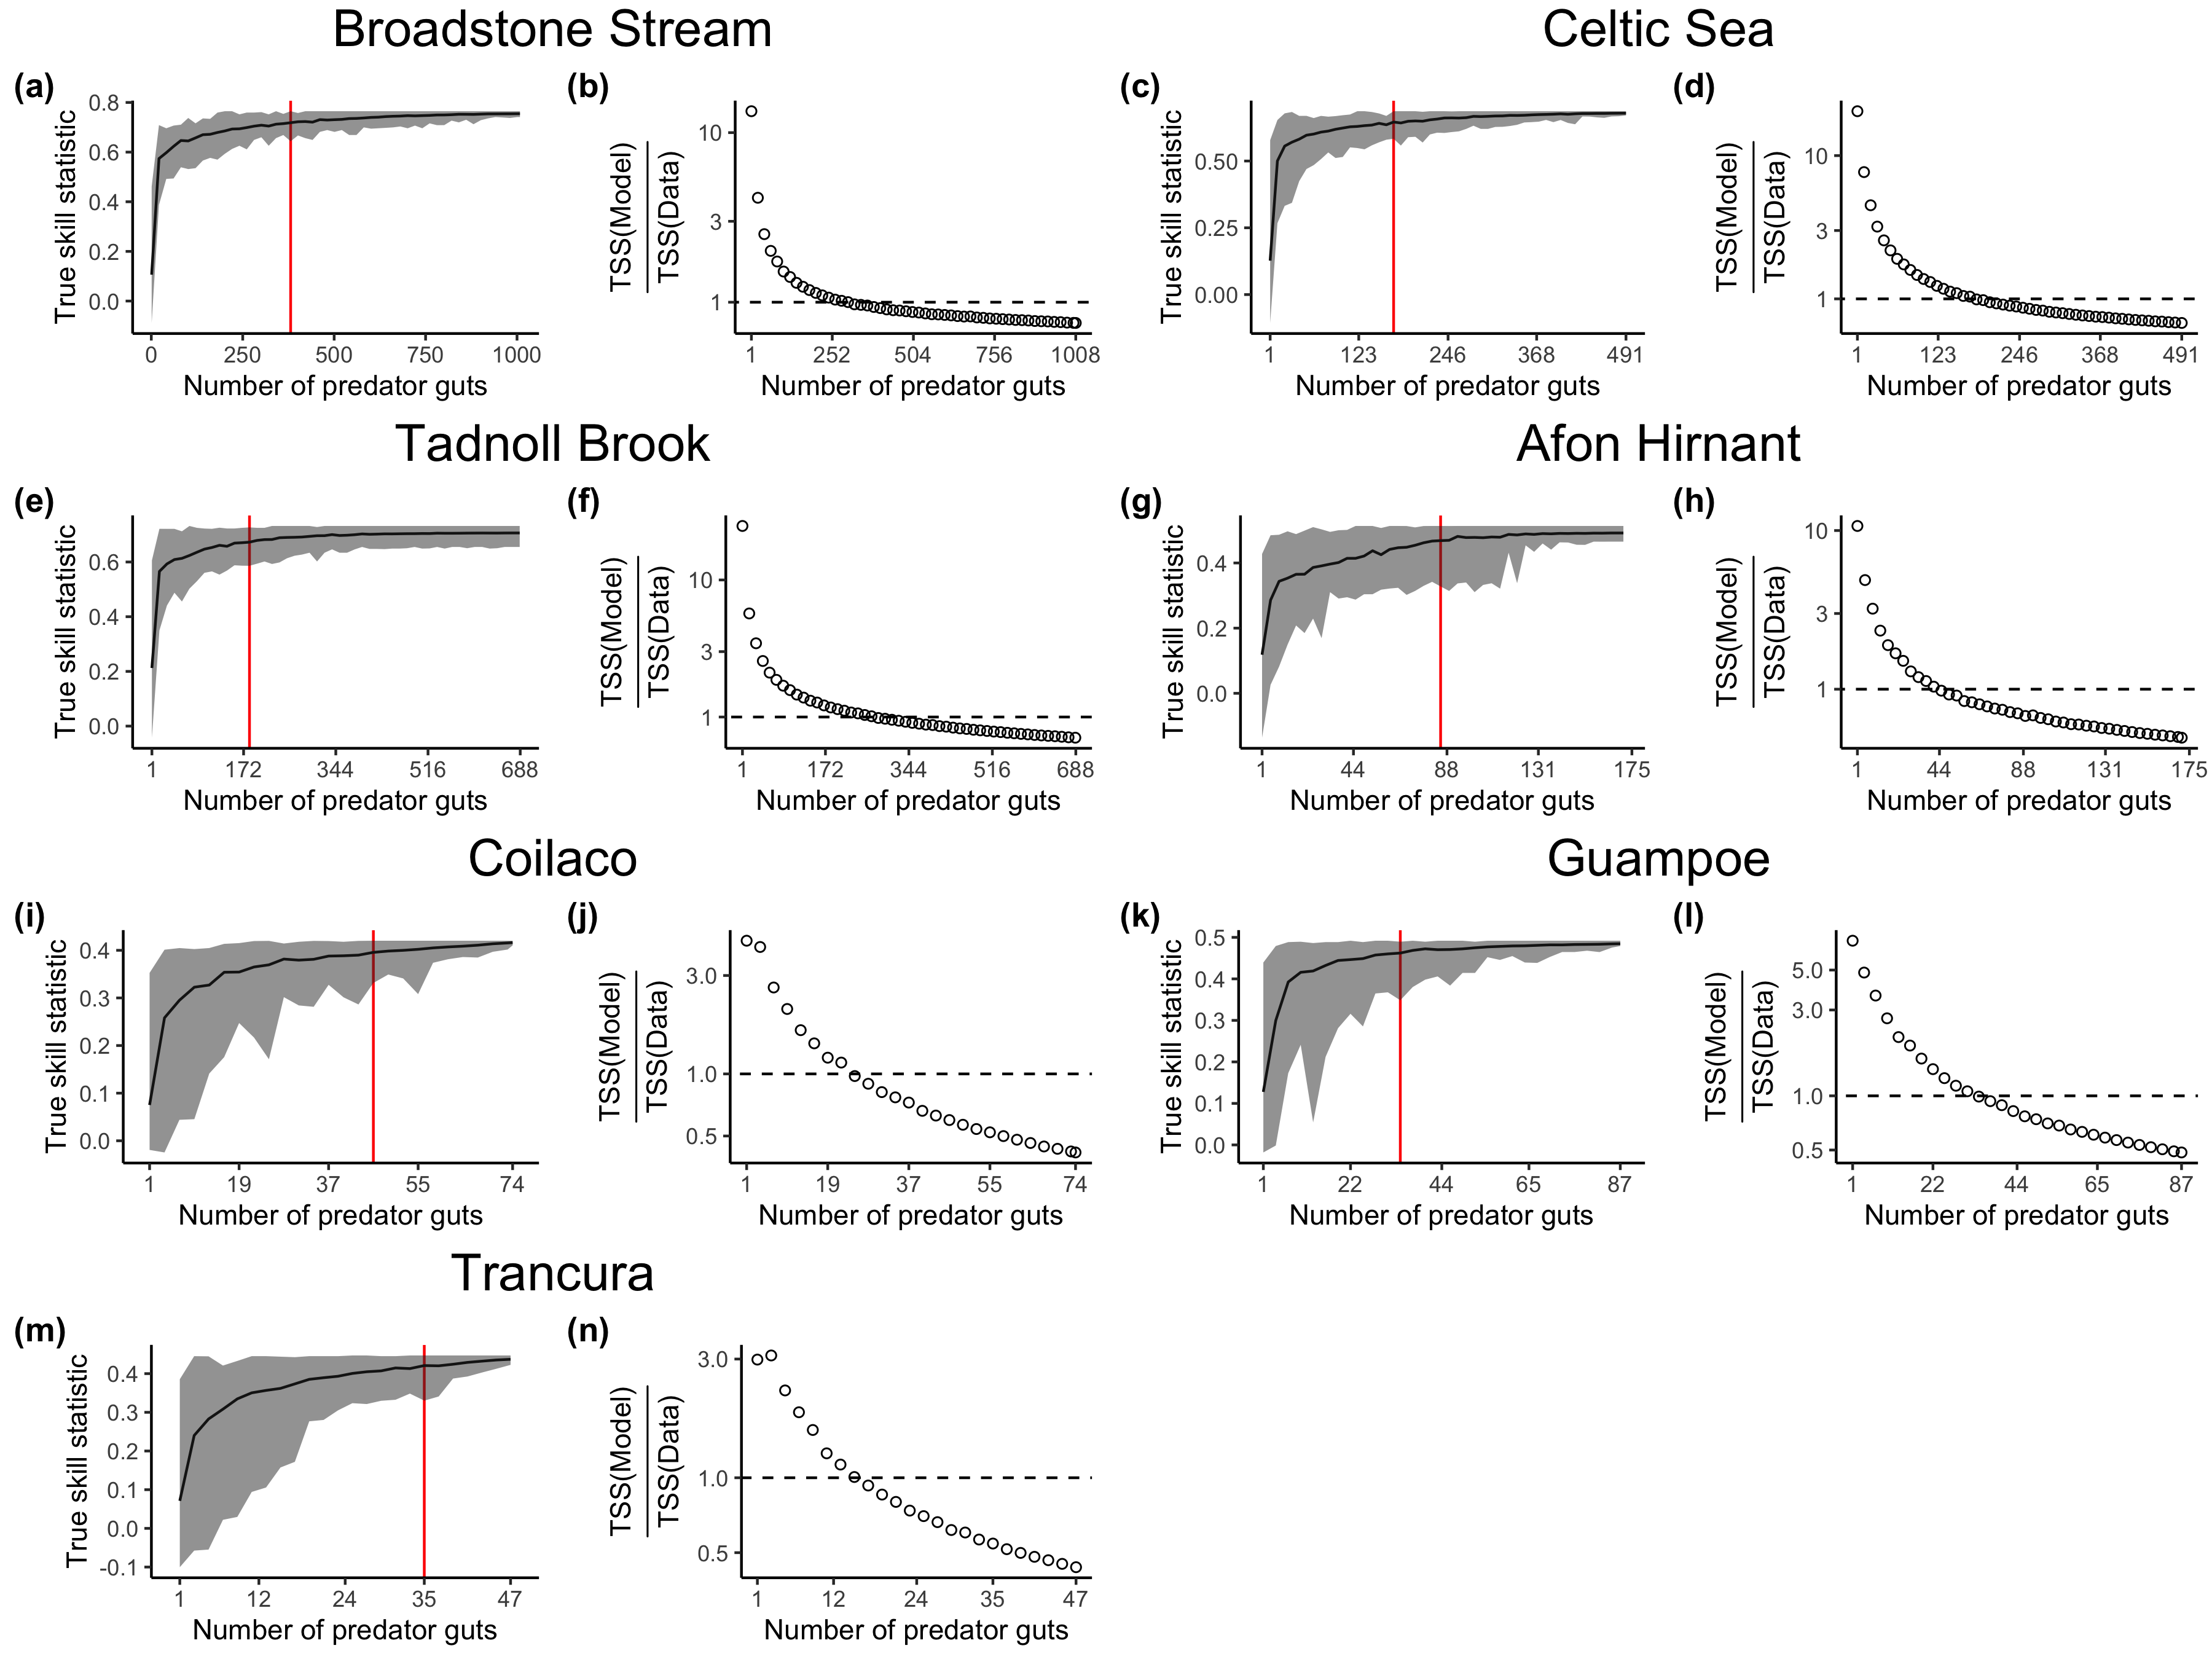
\includegraphics[width=500px]{../../results/misc/plot_TSS_ratio} 

}

\caption{\label{fig:fig_ra} (a, c, e, g, i, k, m) Accuracy of the predicted food web measured using the true skill statistics, predicted by the ADBM parameterised using gut content data. Line and shaded grey region represents the mean and the prediction interval of 100 independent samples respectively. Red line represents the number of predator guts required to achieve a TSS of 95\% of the maximum TSS. (b, d, f, h, j, l, n) Ratio of the true skill statistic of the predicted food web by the ADBM parameterised using gut content data to that of the predicted food web constructed using gut content data only. The dashed line shows where the ratio is one for reference.}\label{fig:unnamed-chunk-2}
\end{figure}

The true skill statistics of the food webs predicted by the ADBM using
subsets of gut content data improved quickly for lower number of
predator guts (Fig. \ref{fig:fig_ra}) (a, c, e, g, i, k, m).
Furthermore, the width of the prediction interval of the true skill
statistics decreased with increasing number of predator guts with the
mean TSS asymptoting to the maximum mean TSS achieved by the ADBM when
all the gut content data was used. Although the maximum TSS varied among
the food webs, the qualitative increase in the TSS was the same.

For Broadstone Stream food web, with only 381 gut contents, which is
38\% of the total gut content data, the ADBM predicted the food web with
the mean TSS of 0.74 which was 95\% of the mean TSS (0.78) achieved
using complete gut content data (Fig. \ref{fig:fig_ra}(a)). In case of
the Celtic Sea food web, only 171 gut content data which is 35\% of the
total gut content data was required by the ADBM to predict food web with
TSS equal to 95\% of the mean TSS (0.68) achieved using complete gut
content data (Fig. \ref{fig:fig_ra}(c)).

For a low number of predator guts, the TSS of the model predicted food
web was higher than the TSS of the food web constructed from gut content
data only (Fig. \ref{fig:fig_ra} (b, d, f, h, j, l, n)). An increase in
the number of predator guts did reduce the ratio TSS(Model)/TSS(data)
reduced to less than one, and reduced further gradually. This shows that
with less data available it is better to use the model, while if more
data is available then it is better to use the data itself.

\hypertarget{dependence-of-the-minimum-gut-content-data-on-number-of-links-and-connectance}{%
\subsection{Dependence of the minimum gut content data on number of
links and
connectance}\label{dependence-of-the-minimum-gut-content-data-on-number-of-links-and-connectance}}

There was a significant positive relationship between the minimum number
of gut content data (i.e the amount of gut content data used in order to
ensure 95\% of the maximum TSS) and the connectance of the food webs
(Fig. \ref{fig:fig_rb} (a)). Similarly, we also observed a positive
relationship between the minimum number of gut content data and the
number of trophic links (L) in the food webs, however this relationship
was not significant (Fig. \ref{fig:fig_rb} (b)). Furthermore, there was
a significant positive relationship between the number of minimum gut
content data and the the number of maximum gut content data sampled
(Fig. \ref{fig:fig_rb} (c)) for food webs.

\begin{figure}

{\centering 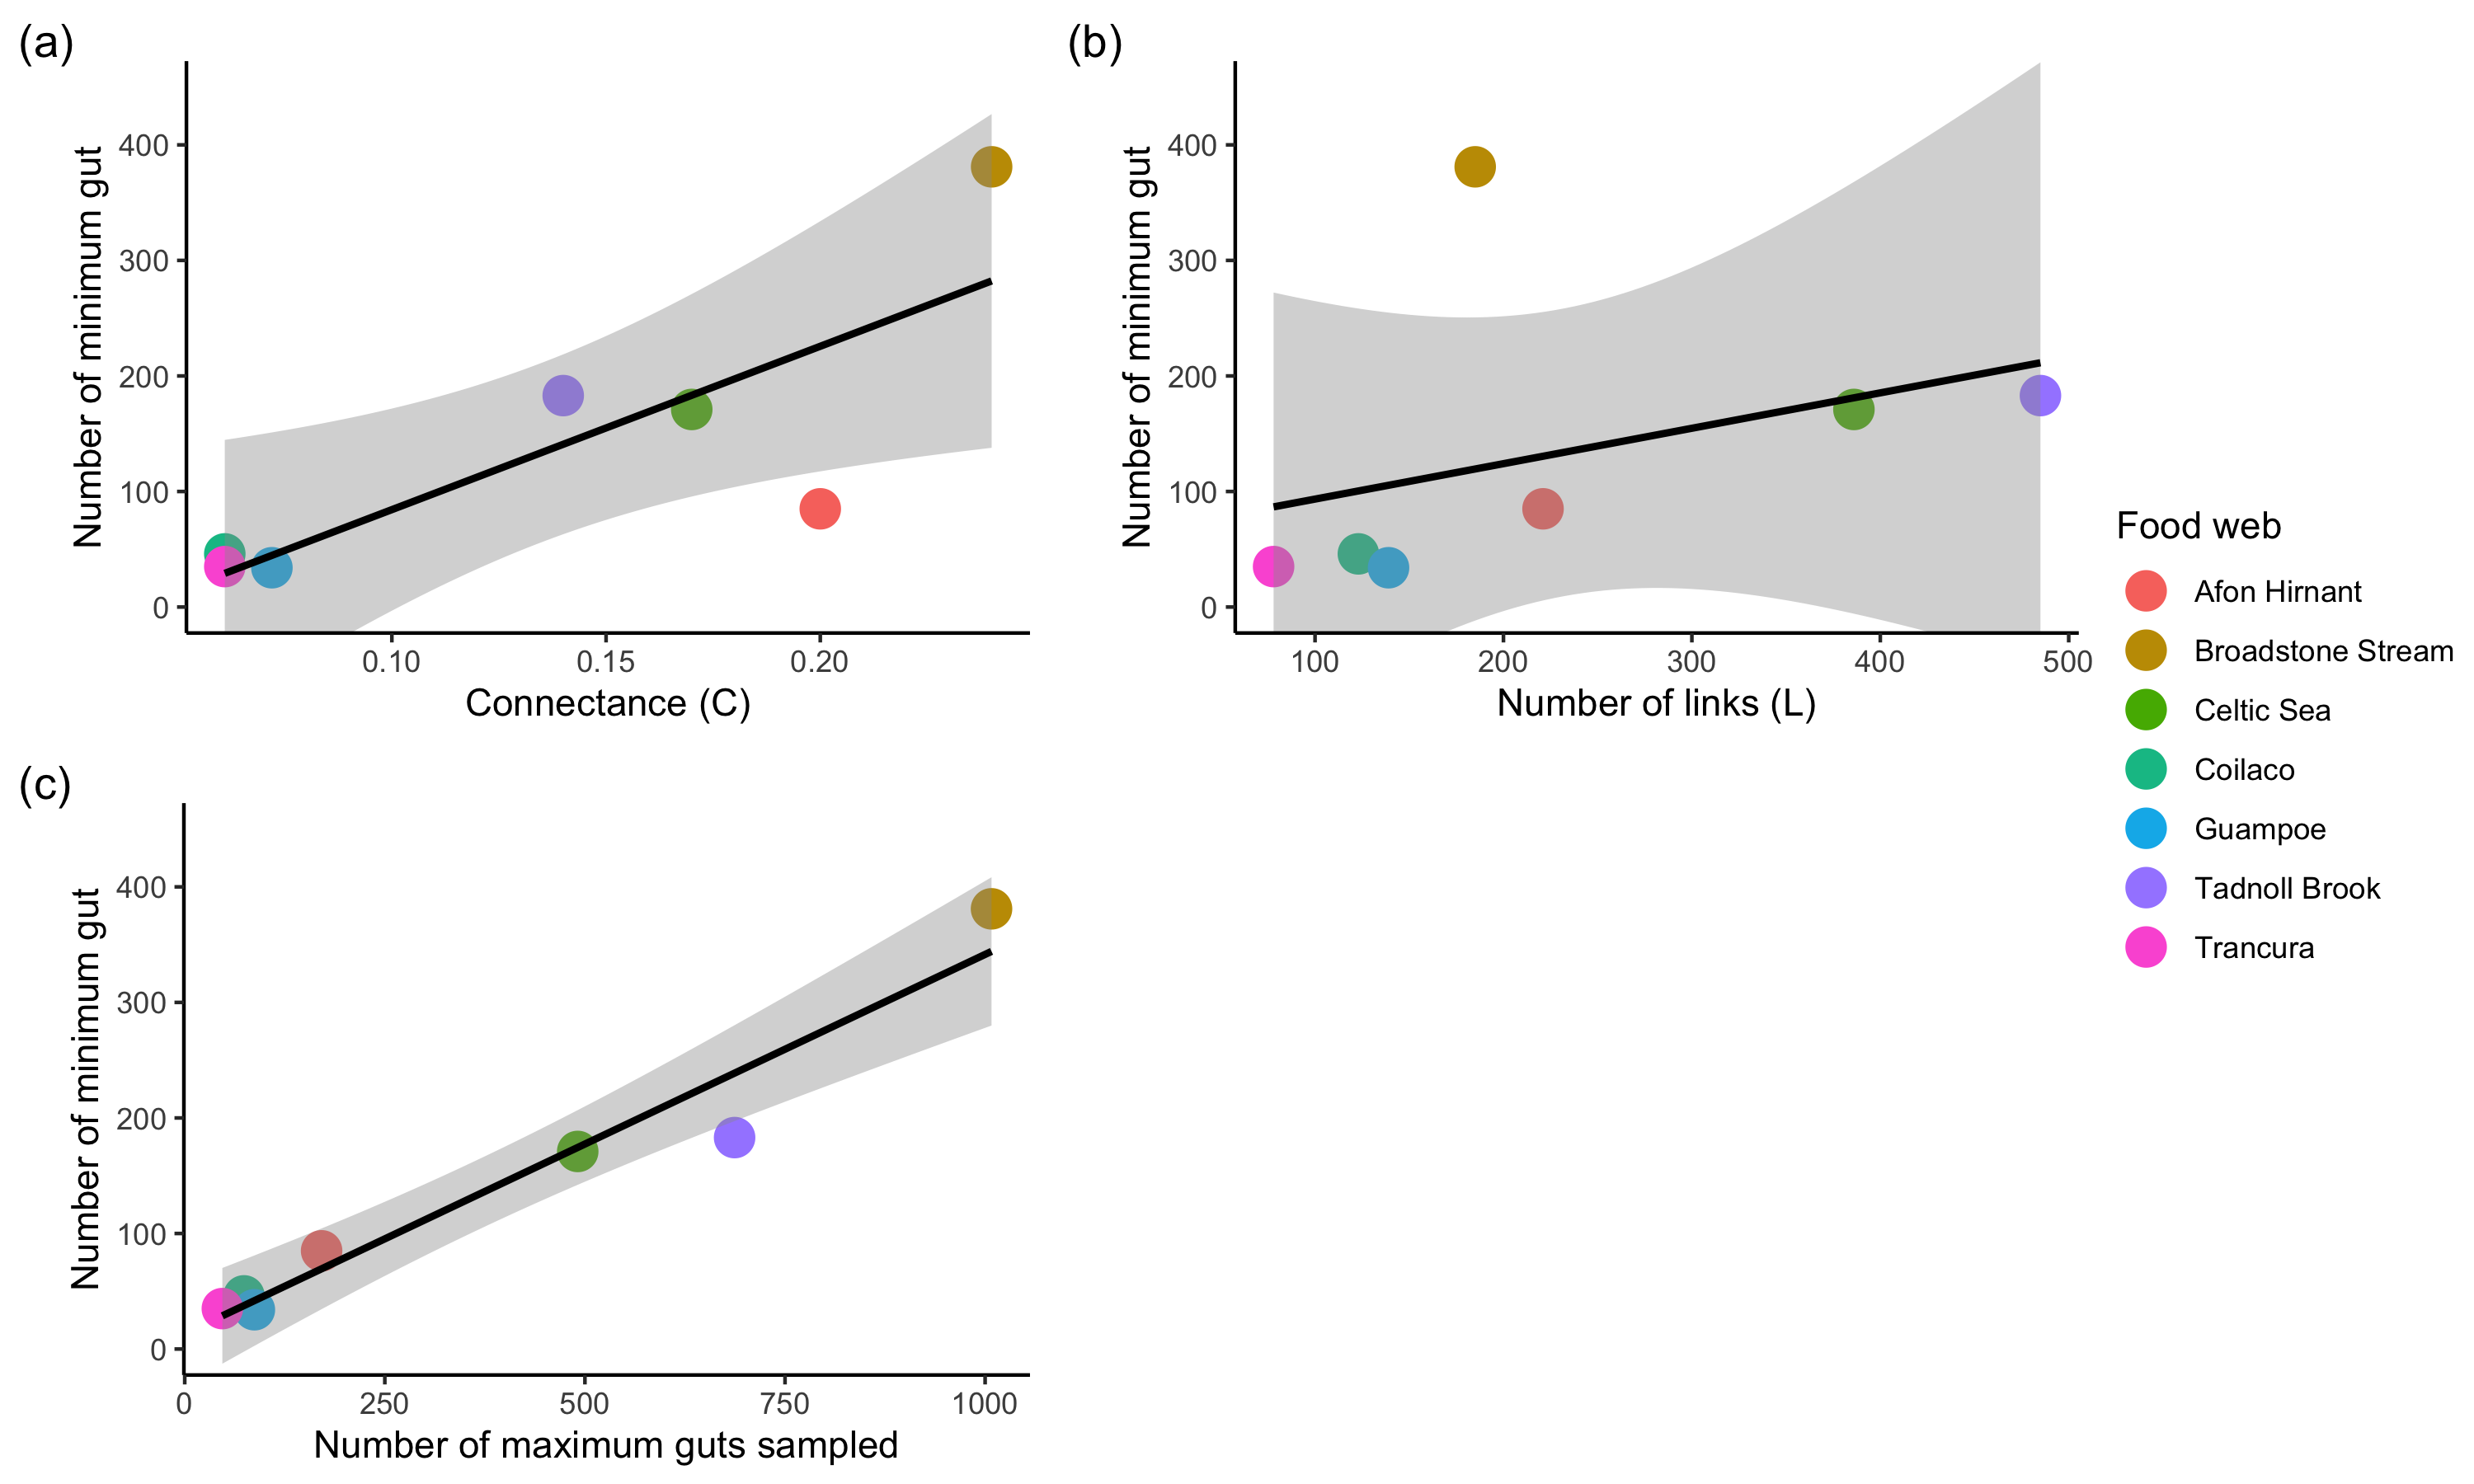
\includegraphics[width=400px]{../../results/misc/plot_min_gut_vs_X} 

}

\caption{\label{fig:fig_rb} (a, b, c) Number of minimum gut content data (i.e the amount of gut content data used in order to ensure 95\% of the maximum TSS) plotted against number of links (L), connectance (C) and number of maximum guts sampled respectively. Solid lines are linear regression ((a) t = 3.138, df = 5, P = 0.0257; (b) t = 0.876, df = 5, P = 0.421; (c) t = 9.571, df = 5, P = 0.0002) and grey region represents 95\% confidence intervals.}\label{fig:unnamed-chunk-3}
\end{figure}

\hypertarget{discussion}{%
\section{Discussion}\label{discussion}}

We have demonstrated how a food web model can be used to predict food
webs reasonably well even when incomplete data about trophic
interactions is available. At lower amount of gut content data,
predicting with the model is better than using the data itself, while at
higher amounts of gut content data, it is better to only use the data.
This can help inform how much gut content data to actually collect when
we are using a food web model to infer trophic interactions. A future
development could be to make the same assessment using other food web
models, and to also use food web data other than gut content data to
parameterise those models.

\hypertarget{why-incomplete-gut-content-data-can-be-used-to-infer-trophic-interactions}{%
\subsection{Why incomplete gut content data can be used to infer trophic
interactions?}\label{why-incomplete-gut-content-data-can-be-used-to-infer-trophic-interactions}}

In all of the seven food webs, the ADBM was able to infer the trophic
interactions using incomplete gut content data because the presence
absence information from the gut content data was still sufficient to
constrain the possible model parameter values of the ADBM that best
explained the predators' diets. Although in theory the ADBM can predict
trophic interactions using only body sizes of organisms as it is based
on set of foraging rule, it still requires some presence absence data to
constrain the posterior parameter space thereby making more accurate
predictions.

\hypertarget{why-does-the-minimum-gut-data-differ-among-food-webs}{%
\subsection{Why does the minimum gut data differ among food
webs?}\label{why-does-the-minimum-gut-data-differ-among-food-webs}}

We found the minimum amount of gut content data to vary across food webs
and this could be due to the possibility that the food webs are sampled
differently, i.e.~some food webs are more extensively sampled than
others (SI Fig. S2). Furthermore, it is possible that interactions in
some of the food webs are are more size-structured than others, and are
therefore better predicted by the ADBM and consequently require a lower
number of gut content data for model parameterisation.

\hypertarget{model-fills-up-missing-interactions-and-guides-sampling-direction}{%
\subsection{Model fills up missing interactions and guides sampling
direction}\label{model-fills-up-missing-interactions-and-guides-sampling-direction}}

When little data about trophic interactions is available, the model can
be used to add data about interactions for which data is missing.
Furthermore, the model predictions can be used as a guide to sample
those predator guts for which we do not have enough information on the
presence of interactions from the empirical gut content samples but the
model suggests there are interactions. Therefore, with enough number of
predator guts sampled one might possibly observe those missed
interactions.

\hypertarget{why-is-models-tss-less-than-one}{%
\subsection{Why is model's TSS less than
one?}\label{why-is-models-tss-less-than-one}}

The food web model used (the ADBM) cannot explain all the interactions
in any observed food web that it has been fit to. The foraging rules it
encodes are based on the body size and have particular structure and
assumptions; not all of these are met by all observed interactions. For
example, the ADBM can only predict diets that are contiguous with
respect to the size of prey. I.e. it cannot predict that a predator will
consume taxa of size 1 and 3, and not taxa of size 2. Hence, if the
observed diets are not contiguous when prey are ordered by their size,
the estimation process could lead to a lower value of the TSS.

Furthermore, the observed data may be missing links, e.g.~links that
rarely occur. Hence the ADBM's maximum predicted true skill statistics
is less than one for all food webs it has so far been fit to.

\hypertarget{tssmodeltssdata-for-different-food-webs}{%
\subsection{TSS(Model)/TSS(Data) for different food
webs}\label{tssmodeltssdata-for-different-food-webs}}

In all the food webs, the ratio TSS(Model)/TSS(Data) decreased with
increasing number of predator guts (Fig. \ref{fig:fig_ra} (b, d, f, h,
j, l, n)). This suggests when less data is available it is better to use
the model and when more data is available it is better to only use the
data to predict trophic interactions. At lower number of predator guts
the model fills up the missing interactions that were not observed in
the gut content data, therefore resulting in model performing better as
compared to data alone. Wile at higher number of predator guts the model
is probably predicting some presence or absence of links i.e.~false
positives and false negatives resulting in a lower TSS as compared to
that of data alone.

\hypertarget{propagating-uncertainty-from-gut-content-data-to-models-predictions}{%
\subsection{Propagating uncertainty from gut content data to model's
predictions}\label{propagating-uncertainty-from-gut-content-data-to-models-predictions}}

There is considerable uncertainty involved in gut content analysis
(Baker, Buckland, and Sheaves 2014) such as in fish's guts, there are
sometimes loose tissues that are not identifiable and cannot be assigned
to a specific prey item with certainty. There are factors such as sample
size of consumers, mechanical prey handling, differential digestion and
evacuation rates of different prey types and volumes, and the ingestion
order that in combination result in an unquantifiable error which is
difficult to interpret in the predator diet (Hyslop 1980; Rindorf and
Lewy 2004; Baker, Buckland, and Sheaves 2014). Therefore, a future
development would be to consider how this uncertainty is propagated into
food web prediction.

\hypertarget{comparing-our-study-with-other-studies-of-predicting-food-webs-using-incomplete-data}{%
\subsection{Comparing our study with other studies of predicting food
webs using incomplete
data}\label{comparing-our-study-with-other-studies-of-predicting-food-webs-using-incomplete-data}}

Some studies have presented how the accuracy of food web prediction
change when we vary the amount of food web data (Gray et al. 2015). For
example: Desjardins-Proulx et al. (2017) has used predictive machine
learning models and Caron et al. (2022) has used predictive traits-based
models on partial knowledge of interactions to reconstruct a food web
accurately, in contrast to our study where we used a mechanistic food
web model.

\hypertarget{what-is-the-generalisability-of-our-results}{%
\subsection{What is the generalisability of our
results?}\label{what-is-the-generalisability-of-our-results}}

In our study, we have implemented the approach only with the ADBM.
However, in principle, this approach could be extended to other food web
models such as (Williams and Martinez 2000; Gravel et al. 2013;
Allesina, Alonso, and Pascual 2008). A future prospect could be to study
how well different food web models' prediction accuracy vary with
different amount of gut content data. This can also help in making
decision as to which food web model to chose from for a given a set of
gut content data. We suspect the relationship (i.e shape of the curve)
between the TSS of the predicted food web and the number of predator
guts might vary within food web models.

\hypertarget{assumption-that-the-food-web-constructed-with-the-total-gut-content-data-is-the-true-food-web-and-how-can-this-be-improved}{%
\subsection{Assumption that the food web constructed with the total gut
content data is the true food web and how can this be
improved}\label{assumption-that-the-food-web-constructed-with-the-total-gut-content-data-is-the-true-food-web-and-how-can-this-be-improved}}

Some of the food webs are not very well predicted using the ADBM. And
this could possibly result in a lower value of minimum gut content data
that was used to achieve 95\% of the maximum TSS. This could be because
our study is based on the assumption that the true food webs is the one
which was constructed using the total gut content data. However, if the
total gut content does not contain sufficient information to construct
the complete food web, then the food web will miss some links. This
would therefore result in a lower TSS of the predicted food web, which
can eventually lead to a lower estimate of the minimum gut content data.
A future prospect could be to incorporate other sources of
presence-absence data such as stable isotope ratio, metabarcoding to
complement any links that were missed by the gut content method.

\hypertarget{how-can-we-include-other-types-of-food-web-data}{%
\subsection{How can we include other types of food web
data?}\label{how-can-we-include-other-types-of-food-web-data}}

A future prospect would be to include other types of food web data along
with gut content simultaneously to parameterise the ADBM. For example,
one could use the approximate trophic position inferred from stable
isotope ratio data from a tissue of an individual and gut content data
of a different predator simultaneously to parameterise a food web model
such as the ADBM. In this case, trophic position would be an additional
summary statistic required in the parameterisation method. This
combination of different types of data about trophic interactions could
be particularly useful when only a limited amount of diet information
can be extracted by using a single method.

\hypertarget{acknowledgements}{%
\section{Acknowledgements}\label{acknowledgements}}

\hypertarget{author-contributions}{%
\section{Author contributions}\label{author-contributions}}

\hypertarget{reference}{%
\section*{Reference}\label{reference}}
\addcontentsline{toc}{section}{Reference}

\hypertarget{refs}{}
\begin{CSLReferences}{1}{0}
\leavevmode\vadjust pre{\hypertarget{ref-allesinaGeneralModelFood2008}{}}%
Allesina, Stefano, David Alonso, and Mercedes Pascual. 2008. {``A
{General Model} for {Food Web Structure}.''} \emph{Science} 320 (5876):
658--61. \url{https://doi.org/10.1126/science.1156269}.

\leavevmode\vadjust pre{\hypertarget{ref-alloucheAssessingAccuracySpecies2006}{}}%
Allouche, Omri, Asaf Tsoar, and Ronen Kadmon. 2006. {``Assessing the
Accuracy of Species Distribution Models: Prevalence, Kappa and the True
Skill Statistic ({TSS}).''} \emph{Journal of Applied Ecology} 43 (6):
1223--32. \url{https://doi.org/10.1111/j.1365-2664.2006.01214.x}.

\leavevmode\vadjust pre{\hypertarget{ref-bakerFishGutContent2014}{}}%
Baker, Ronald, Amanda Buckland, and Marcus Sheaves. 2014. {``Fish Gut
Content Analysis: Robust Measures of Diet Composition.''} \emph{Fish and
Fisheries} 15 (1): 170--77. \url{https://doi.org/10.1111/faf.12026}.

\leavevmode\vadjust pre{\hypertarget{ref-barnesPredatorPreyBody2008}{}}%
Barnes, C., D. M. Bethea, R. D. Brodeur, J. Spitz, V. Ridoux, C.
Pusineri, B. C. Chase, et al. 2008. {``Predator and {Prey Body Sizes} in
{Marine Food Webs}.''} \emph{Ecology} 89 (3): 881--81.
\url{https://doi.org/10.1890/07-1551.1}.

\leavevmode\vadjust pre{\hypertarget{ref-baumgartnerPredictiveLengthDry2003}{}}%
Baumgärtner, Daniel, and Karl-Otto Rothhaupt. 2003. {``Predictive
{Length}--{Dry Mass Regressions} for {Freshwater Invertebrates} in a
{Pre-Alpine Lake Littoral}.''} \emph{International Review of
Hydrobiology} 88 (5): 453--63.
\url{https://doi.org/10.1002/iroh.200310632}.

\leavevmode\vadjust pre{\hypertarget{ref-benkeLengthMassRelationshipsFreshwater1999}{}}%
Benke, Arthur C., Alexander D. Huryn, Leonard A. Smock, and J. Bruce
Wallace. 1999. {``Length-{Mass Relationships} for {Freshwater
Macroinvertebrates} in {North America} with {Particular Reference} to
the {Southeastern United States}.''} \emph{Journal of the North American
Benthological Society} 18 (3): 308--43.
\url{https://doi.org/10.2307/1468447}.

\leavevmode\vadjust pre{\hypertarget{ref-blanchardClimateFishingInfluence2005}{}}%
Blanchard, Julia L., Nicholas K. Dulvy, Simon Jennings, James R. Ellis,
John K. Pinnegar, Alex Tidd, and Laurence T. Kell. 2005. {``Do Climate
and Fishing Influence Size-Based Indicators of {Celtic Sea} Fish
Community Structure?''} \emph{ICES Journal of Marine Science} 62 (3):
405--11. \url{https://doi.org/10.1016/j.icesjms.2005.01.006}.

\leavevmode\vadjust pre{\hypertarget{ref-burgherrRegressionAnalysisLinear1997}{}}%
Burgherr, Peter, and Elisabeth I. Meyer. 1997. {``Regression Analysis of
Linear Body Dimensions Vs. Dry Mass in Stream Macroinvertebrates.''}
\emph{Archiv Für Hydrobiologie}, April, 101--12.
\url{https://doi.org/10.1127/archiv-hydrobiol/139/1997/101}.

\leavevmode\vadjust pre{\hypertarget{ref-caronAddressingEltonianShortfall}{}}%
Caron, Dominique, Luigi Maiorano, Wilfried Thuiller, and Laura J.
Pollock. 2022. {``Addressing the {Eltonian} Shortfall with Trait-Based
Interaction Models.''} \emph{Ecology Letters} n/a (n/a).
\url{https://doi.org/10.1111/ele.13966}.

\leavevmode\vadjust pre{\hypertarget{ref-cohenSoilInvertebratesChemistry2014}{}}%
Cohen, Joel E., and Christian Mulder. 2014a. {``Soil Invertebrates,
Chemistry, Weather, Human Management, and Edaphic Food Webs at 135 Sites
in {The Netherlands}: {SIZEWEB}.''} \emph{Ecology} 95 (2): 578--78.
\url{https://doi.org/10.1890/13-1337.1}.

\leavevmode\vadjust pre{\hypertarget{ref-cohen2014}{}}%
---------. 2014b. {``Soil Invertebrates, Chemistry, Weather, Human
Management, and Edaphic Food Webs at 135 Sites in The Netherlands:
SIZEWEB.''} \emph{Ecology} 95 (2): 578--78.
\url{https://doi.org/10.1890/13-1337.1}.

\leavevmode\vadjust pre{\hypertarget{ref-cohenStochasticTheoryCommunity1985}{}}%
Cohen, Joel E., C. M. Newman, and John Hyslop Steele. 1985. {``A
Stochastic Theory of Community Food Webs {I}. {Models} and Aggregated
Data.''} \emph{Proceedings of the Royal Society of London. Series B.
Biological Sciences} 224 (1237): 421--48.
\url{https://doi.org/10.1098/rspb.1985.0042}.

\leavevmode\vadjust pre{\hypertarget{ref-crawfordApplicationsStableIsotope2008}{}}%
Crawford, Kerry, Robbie A. Mcdonald, and Stuart Bearhop. 2008.
{``Applications of Stable Isotope Techniques to the Ecology of
Mammals.''} \emph{Mammal Review} 38 (1): 87--107.
\url{https://doi.org/10.1111/j.1365-2907.2008.00120.x}.

\leavevmode\vadjust pre{\hypertarget{ref-desjardins-proulxEcologicalInteractionsNetflix2017}{}}%
Desjardins-Proulx, Philippe, Idaline Laigle, Timoth'ee Poisot, and
Dominique Gravel. 2017. {``Ecological Interactions and the {Netflix}
Problem.''} \emph{PeerJ} 5 (August): e3644.
\url{https://doi.org/10.7717/peerj.3644}.

\leavevmode\vadjust pre{\hypertarget{ref-dunneNetworkStructureBiodiversity2002}{}}%
Dunne, Jennifer A., Richard J. Williams, and Neo D. Martinez. 2002.
{``Network Structure and Biodiversity Loss in Food Webs: Robustness
Increases with Connectance.''} \emph{Ecology Letters} 5 (4): 558--67.
\url{https://doi.org/10.1046/j.1461-0248.2002.00354.x}.

\leavevmode\vadjust pre{\hypertarget{ref-edwardsRelationshipLengthMass2009}{}}%
Edwards, François K. Lauridsen, Lucie Armand, Helen M. Vincent, and Iwan
J. Jones. 2009. {``The Relationship Between Length, Mass and
Preservation Time for Three Species of Freshwater Leeches
({Hirudinea}).''} \emph{Fundamental and Applied Limnology} 173 (4):
321--27. \url{https://doi.org/10.1127/1863-9135/2009/0173-0321}.

\leavevmode\vadjust pre{\hypertarget{ref-figueroaFoodWebDynamics2007}{}}%
Figueroa, David. 2007. {``Food Web Dynamics : New Patterns from Southern
{South America} and {North Wales UK}, and the Role of Basal Species
Structuring Food Webs.''} PhD thesis, {University of London}.
\url{https://ethos.bl.uk/OrderDetails.do?uin=uk.bl.ethos.582554}.

\leavevmode\vadjust pre{\hypertarget{ref-ganiharBiomassEstimatesTerrestrial1997}{}}%
Ganihar, S. R. 1997. {``Biomass Estimates of Terrestrial Arthropods
Based on Body Length.''} \emph{Journal of Biosciences} 22 (2): 219--24.
\url{https://doi.org/10.1007/BF02704734}.

\leavevmode\vadjust pre{\hypertarget{ref-gilljamSeeingDouble2011}{}}%
Gilljam, David, Aaron Thierry, Francois K. Edwards, David Figueroa,
Anton T. Ibbotson, J. Iwan Jones, Rasmus B. Lauridsen, Owen L. Petchey,
Guy Woodward, and Bo Ebenman. 2011. {``Seeing {Double}:''} In
\emph{Advances in {Ecological Research}}, 45:67--133. {Elsevier}.
\url{https://doi.org/10.1016/B978-0-12-386475-8.00003-4}.

\leavevmode\vadjust pre{\hypertarget{ref-goldwasserConstructionAnalysisLarge1993a}{}}%
Goldwasser, Lloyd, and Jonathan Roughgarden. 1993a. {``Construction and
{Analysis} of a {Large Caribbean Food Web}.''} \emph{Ecology} 74 (4):
1216--33. \url{https://doi.org/10.2307/1940492}.

\leavevmode\vadjust pre{\hypertarget{ref-goldwasser1993}{}}%
---------. 1993b. {``Construction and Analysis of a Large Caribbean Food
Web.''} \emph{Ecology} 74 (4): 1216--33.
\url{https://doi.org/10.2307/1940492}.

\leavevmode\vadjust pre{\hypertarget{ref-gonzalezSizemassRelationshipsStream}{}}%
Gonzalez, Jose M, Ana Basaguren, and Jesus Pozo. 2002. {``Size-Mass
Relationships of Stream Invertebrates in a Northern {Spain} Stream,''}
7.

\leavevmode\vadjust pre{\hypertarget{ref-ogormanSimpleModelPredicts2019}{}}%
Gorman, Eoin J. O', Owen L. Petchey, Katy J. Faulkner, Bruno Gallo,
Timothy A. C. Gordon, Joana Neto-Cerejeira, J'on S. 'Olafsson, Doris E.
Pichler, Murray S. A. Thompson, and Guy Woodwar. 2019. {``A Simple Model
Predicts How Warming Simplifies Wild Food Webs.''} \emph{Nature Climate
Change} 9 (8, 8): 611--16.
\url{https://doi.org/10.1038/s41558-019-0513-x}.

\leavevmode\vadjust pre{\hypertarget{ref-gravelInferringFoodWeb2013}{}}%
Gravel, Dominique, Timoth'ee Poisot, Camille Albouy, Laure Velez, and
David Mouillot. 2013. {``Inferring Food Web Structure from Predator-Prey
Body Size Relationships.''} Edited by Robert Freckleton. \emph{Methods
in Ecology and Evolution} 4 (11): 1083--90.
\url{https://doi.org/10.1111/2041-210X.12103}.

\leavevmode\vadjust pre{\hypertarget{ref-grayJoiningDotsAutomated2015}{}}%
Gray, Clare, David H. Figueroa, Lawrence N. Hudson, Athen Ma, Dan
Perkins, and Guy Woodward. 2015. {``Joining the Dots: {An} Automated
Method for Constructing Food Webs from Compendia of Published
Interactions.''} \emph{Food Webs} 5 (December): 11--20.
\url{https://doi.org/10.1016/j.fooweb.2015.09.001}.

\leavevmode\vadjust pre{\hypertarget{ref-guptaSimultaneouslyEstimatingFood2022}{}}%
Gupta, Anubhav, Reinhard Furrer, and Owen L. Petchey. 2022.
{``Simultaneously Estimating Food Web Connectance and Structure with
Uncertainty.''} \emph{Ecology and Evolution} 12 (3): e8643.
\url{https://doi.org/10.1002/ece3.8643}.

\leavevmode\vadjust pre{\hypertarget{ref-hattabForecastingFinescaleChanges2016}{}}%
Hattab, Tarek, Fabien Leprieur, Frida Ben Rais Lasram, Dominique Gravel,
François Le Loc'h, and Camille Albouy. 2016. {``Forecasting Fine-Scale
Changes in the Food-Web Structure of Coastal Marine Communities Under
Climate Change.''} \emph{Ecography} 39 (12): 1227--37.
\url{https://doi.org/10.1111/ecog.01937}.

\leavevmode\vadjust pre{\hypertarget{ref-hyslopStomachContentsAnalysis1980}{}}%
Hyslop, E. J. 1980. {``Stomach Contents Analysis---a Review of Methods
and Their Application.''} \emph{Journal of Fish Biology} 17 (4):
411--29. \url{https://doi.org/10.1111/j.1095-8649.1980.tb02775.x}.

\leavevmode\vadjust pre{\hypertarget{ref-jenningsTrophicLevelsMarine2015}{}}%
Jennings, Simon, and Johan van der Molen. 2015. {``Trophic Levels of
Marine Consumers from Nitrogen Stable Isotope Analysis: Estimation and
Uncertainty.''} \emph{ICES Journal of Marine Science} 72 (8):
2289--2300. \url{https://doi.org/10.1093/icesjms/fsv120}.

\leavevmode\vadjust pre{\hypertarget{ref-jordanKeystoneSpeciesFood2009}{}}%
Jord'an, Ferenc. 2009. {``Keystone Species and Food Webs.''}
\emph{Philosophical Transactions of the Royal Society B: Biological
Sciences} 364 (1524): 1733--41.
\url{https://doi.org/10.1098/rstb.2008.0335}.

\leavevmode\vadjust pre{\hypertarget{ref-kadoyaIsoWebBayesianIsotope2012}{}}%
Kadoya, Taku, Yutaka Osada, and Gaku Takimoto. 2012. {``{IsoWeb}: {A
Bayesian Isotope Mixing Model} for {Diet Analysis} of the {Whole Food
Web}.''} Edited by Simon Thrush. \emph{PLoS ONE} 7 (7): e41057.
\url{https://doi.org/10.1371/journal.pone.0041057}.

\leavevmode\vadjust pre{\hypertarget{ref-kellyUsingEnvironmentalDNA2014}{}}%
Kelly, Ryan P., Jesse A. Port, Kevan M. Yamahara, and Larry B. Crowder.
2014. {``Using {Environmental DNA} to {Census Marine Fishes} in a {Large
Mesocosm}.''} \emph{PLOS ONE} 9 (1): e86175.
\url{https://doi.org/10.1371/journal.pone.0086175}.

\leavevmode\vadjust pre{\hypertarget{ref-laymanCanStableIsotope2007}{}}%
Layman, Craig A., D. Albrey Arrington, Carmen G. Montaña, and David M.
Post. 2007. {``Can {Stable Isotope Ratios Provide} for {Community}-{Wide
Measures} of {Trophic Structure}?''} \emph{Ecology} 88 (1): 42--48.
\url{https://doi.org/10.1890/0012-9658(2007)88\%5B42:CSIRPF\%5D2.0.CO;2}.

\leavevmode\vadjust pre{\hypertarget{ref-lindegrenEcologicalForecastingClimate2010}{}}%
Lindegren, Martin, Christian Möllmann, Anders Nielsen, Keith Brander,
Brian R. MacKenzie, and Nils Chr. Stenseth. 2010. {``Ecological
Forecasting Under Climate Change: The Case of {Baltic} Cod.''}
\emph{Proceedings of the Royal Society B: Biological Sciences} 277
(1691): 2121--30. \url{https://doi.org/10.1098/rspb.2010.0353}.

\leavevmode\vadjust pre{\hypertarget{ref-macarthurOptimalUsePatchy1966}{}}%
MacArthur, Robert H., and Eric R. Pianka. 1966. {``On {Optimal Use} of a
{Patchy Environment}.''} \emph{The American Naturalist} 100 (916):
603--9. \url{https://www.jstor.org/stable/2459298}.

\leavevmode\vadjust pre{\hypertarget{ref-meyerRelationshipBodyLength1989}{}}%
MEYER, E. 1989. {``The Relationship Between Body Length Parameters and
Dry Mass in Running Water Invertebrates.''} \emph{Arch Hydrobiol} 117:
191--203. \url{https://ci.nii.ac.jp/naid/10019557615/}.

\leavevmode\vadjust pre{\hypertarget{ref-miserendinoRelacionesLongitudpesoPara2001}{}}%
Miserendino, Mar'ıa L. 2001. {``Relaciones Longitud-Peso Para
Macroinvertebrados de Ambientes Dulceacuícolas de {Patagonia}
({Argentina}).''} \emph{Ecología Austral} 11 (1): 3--8.
\url{http://www.scielo.org.ar/scielo.php?script=sci_abstract\&pid=S1667-782X2001000100002\&lng=es\&nrm=iso\&tlng=es}.

\leavevmode\vadjust pre{\hypertarget{ref-nielsen2018}{}}%
Nielsen, Jens M., Elizabeth L. Clare, Brian Hayden, Michael T. Brett,
and Pavel Kratina. 2018. {``Diet Tracing in Ecology: Method Comparison
and Selection.''} Edited by M. Thomas P. Gilbert. \emph{Methods in
Ecology and Evolution} 9 (2): 278--91.
\url{https://doi.org/10.1111/2041-210X.12869}.

\leavevmode\vadjust pre{\hypertarget{ref-peralta-maraverStructureDynamicsStability2017}{}}%
Peralta-Maraver, I., M. J. Lopez-Rodriguez, and J. M. Tierno de
Figueroa. 2017. {``Structure, Dynamics and Stability of a
{Mediterranean} River Food Web.''} \emph{Marine and Freshwater Research}
68 (3): 484--95. \url{https://doi.org/10.1071/MF15154}.

\leavevmode\vadjust pre{\hypertarget{ref-petcheySizeForagingFood2008}{}}%
Petchey, Owen L., Andrew P. Beckerman, Jens O. Riede, and Philip H.
Warren. 2008. {``Size, Foraging, and Food Web Structure.''}
\emph{Proceedings of the National Academy of Sciences} 105: 4191--96.
\url{https://doi.org/10.1073/pnas.0710672105}.

\leavevmode\vadjust pre{\hypertarget{ref-pinnegarDoesDietCeltic2003}{}}%
Pinnegar, J. K., V. M. Trenkel, A. N. Tidd, W. A. Dawson, and M. H. Du
buit. 2003. {``Does Diet in {Celtic Sea} Fishes Reflect Prey
Availability?''} \emph{Journal of Fish Biology} 63 (s1): 197--212.
\url{https://doi.org/10.1111/j.1095-8649.2003.00204.x}.

\leavevmode\vadjust pre{\hypertarget{ref-pompanonWhoEatingWhat2012}{}}%
Pompanon, Francois, Bruce E. Deagle, William O. C. Symondson, David S.
Brown, Simon N. Jarman, and Pierre Taberlet. 2012. {``Who Is Eating
What: Diet Assessment Using Next Generation Sequencing.''}
\emph{Molecular Ecology} 21 (8): 1931--50.
\url{https://doi.org/10.1111/j.1365-294X.2011.05403.x}.

\leavevmode\vadjust pre{\hypertarget{ref-reissExistingPlentyAbundance2008}{}}%
Reiss, Julia, and Jenny M. Schmid-Araya. 2008. {``Existing in Plenty:
Abundance, Biomass and Diversity of Ciliates and Meiofauna in Small
Streams.''} \emph{Freshwater Biology} 53 (4): 652--68.
\url{https://doi.org/10.1111/j.1365-2427.2007.01907.x}.

\leavevmode\vadjust pre{\hypertarget{ref-rindorfBiasEstimatingFood2004}{}}%
Rindorf, A, and P Lewy. 2004. {``Bias in Estimating Food Consumption of
Fish by Stomach-Content Analysis''} 61: 12.

\leavevmode\vadjust pre{\hypertarget{ref-roslinUseDNABarcodes2016}{}}%
Roslin, Tomas, and Sanna Majaneva. 2016. {``The Use of {DNA} Barcodes in
Food Web Construction---Terrestrial and Aquatic Ecologists Unite!''}
Edited by Elizabeth Clare. \emph{Genome} 59 (9): 603--28.
\url{https://doi.org/10.1139/gen-2015-0229}.

\leavevmode\vadjust pre{\hypertarget{ref-schmid-arayaConnectanceStreamFood2002}{}}%
Schmid-Araya, Jenny M., Peter E. Schmid, Anne Robertson, Julie
Winterbottom, Charlotte Gjerløv, and Alan G. Hildrew. 2002.
{``Connectance in {Stream Food Webs}.''} \emph{Journal of Animal
Ecology} 71 (6): 1056--62. \url{https://www.jstor.org/stable/1555780}.

\leavevmode\vadjust pre{\hypertarget{ref-smockRelationshipsBodySize1980}{}}%
Smock, Leonard A. 1980. {``Relationships Between Body Size and Biomass
of Aquatic Insects.''} \emph{Freshwater Biology} 10 (4): 375--83.
\url{https://doi.org/10.1111/j.1365-2427.1980.tb01211.x}.

\leavevmode\vadjust pre{\hypertarget{ref-tamaddoni-nezhadConstructionValidationFood2013}{}}%
Tamaddoni-Nezhad, Alireza, Ghazal Afroozi Milani, Alan Raybould, Stephen
Muggleton, and David A. Bohan. 2013. {``Construction and {Validation} of
{Food Webs Using Logic}-{Based Machine Learning} and {Text Mining}.''}
In \emph{Advances in {Ecological Research}}, 49:225--89. {Elsevier}.
\url{https://doi.org/10.1016/B978-0-12-420002-9.00004-4}.

\leavevmode\vadjust pre{\hypertarget{ref-wadaUseStableIsotopes1991}{}}%
Wada, E., H. Mizutani, and M. Minagawa. 1991. {``The Use of Stable
Isotopes for Food Web Analysis.''} \emph{Critical Reviews in Food
Science and Nutrition} 30 (4): 361--71.
\url{https://doi.org/10.1080/10408399109527547}.

\leavevmode\vadjust pre{\hypertarget{ref-warrenSpatialTemporalVariation1989}{}}%
Warren, Philip H. 1989. {``Spatial and {Temporal Variation} in the
{Structure} of a {Freshwater Food Web}.''} \emph{Oikos} 55 (3): 299.
\url{https://doi.org/10.2307/3565588}.

\leavevmode\vadjust pre{\hypertarget{ref-wilkinsonFAIRGuidingPrinciples2016}{}}%
Wilkinson, Mark D., Michel Dumontier, IJsbrand Jan Aalbersberg,
Gabrielle Appleton, Myles Axton, Arie Baak, Niklas Blomberg, et al.
2016. {``The {FAIR Guiding Principles} for Scientific Data Management
and Stewardship.''} \emph{Scientific Data} 3 (1, 1): 160018.
\url{https://doi.org/10.1038/sdata.2016.18}.

\leavevmode\vadjust pre{\hypertarget{ref-williamsSimpleRulesYield2000}{}}%
Williams, Richard J., and Neo D. Martinez. 2000. {``Simple Rules Yield
Complex Food Webs.''} \emph{Nature} 404 (6774, 6774): 180--83.
\url{https://doi.org/10.1038/35004572}.

\leavevmode\vadjust pre{\hypertarget{ref-woodwardIndividualBasedFoodWebs2010}{}}%
Woodward, Guy, Julia Blanchard, Rasmus B. Lauridsen, Francois K.
Edwards, J. Iwan Jones, David Figueroa, Philip H. Warren, and Owen L.
Petchey. 2010b. {``Individual-{Based Food Webs}.''} In \emph{Advances in
{Ecological Research}}, 43:211--66. {Elsevier}.
\url{https://doi.org/10.1016/B978-0-12-385005-8.00006-X}.

\leavevmode\vadjust pre{\hypertarget{ref-woodward2010}{}}%
---------. 2010a. {``Individual-Based Food Webs.''} In, 43:211--66.
Elsevier. \url{https://doi.org/10.1016/B978-0-12-385005-8.00006-X}.

\leavevmode\vadjust pre{\hypertarget{ref-woodwardChapterIndividualBasedFood2010}{}}%
---------. 2010c. {``Chapter 6 - {Individual}-{Based Food Webs}:
{Species Identity}, {Body Size} and {Sampling Effects}.''} In
\emph{Advances in {Ecological Research}}, edited by Guy Woodward,
43:211--66. Integrative {Ecology}: {From Molecules} to {Ecosystems}.
{Academic Press}.
\url{https://doi.org/10.1016/B978-0-12-385005-8.00006-X}.

\leavevmode\vadjust pre{\hypertarget{ref-woodwardBodysizeDeterminantsNiche2002}{}}%
Woodward, Guy, and Alan G. Hildrew. 2002. {``Body-Size Determinants of
Niche Overlap and Intraguild Predation Within a Complex Food Web.''}
\emph{Journal of Animal Ecology} 71 (6): 1063--74.
\url{https://doi.org/10.1046/j.1365-2656.2002.00669.x}.

\leavevmode\vadjust pre{\hypertarget{ref-woodwardQuantificationResolutionComplex2005}{}}%
Woodward, Guy, Dougie C. Speirs, and Alan G. Hildrew. 2005.
{``Quantification and {Resolution} of a {Complex}, {Size}-{Structured
Food Web}.''} In \emph{Advances in {Ecological Research}}, 36:85--135.
{Elsevier}. \url{https://doi.org/10.1016/S0065-2504(05)36002-8}.

\end{CSLReferences}

\bibliographystyle{biblatex}
\bibliography{bibliography.bib}


\end{document}
